\chapter{Третья глава. Цифровая подпись}
\label{cha:ch_3}
\section{Краткий обзор}
Механизм цифровой подписи определяется посредством реализации двух основных процессов:
\begin{itemize}
	\item формирование подписи;
	\item проверка подписи.
\end{itemize}
\par
Цифровая подпись предназначена для аутентификации лица, подписывающего электронное сообщение. Кроме того, использование ЭЦП предоставляет возможность обеспечить следующие свойства при передаче в системе подписанного сообщения:
\begin{itemize}
	\item осуществление контроля целостности передаваемого подписанного сообщения,
	\item доказательное подтверждение авторства лица,
	\item защита сообщения от возможной подделки.
\end{itemize}
\par
Впервые стандарт на цифровую подпись был введен в 1995 году в составе ГОСТ Р 34.10-1994 \cite{GOST34101994}. Процедуры проверки и генерации цифровой подписи в нем основывались на операциях в поле $\mathbb{Z}_p$. Стойкость его алгоритмов основывалась на сложности решения задачи логарифмирования в $\mathbb{Z}_p$ и стойкости функции хэширования, определенной в ГОСТ Р 34.11-1994. Помимо прочего в стандарте указаны процедуры генерации параметров цифровой подписи.
\par
В следующем стандарте ГОСТ Р 34.10-2001 \cite{GOST34102001}, введеном в 2001 году, вопрос обеспечения стойкости был пересмотрен по сравнению с предыдущим стандартом. Стойкость нового алгоритма основывалась на сложности решения задачи дискретного логарифмирования в группе точек эллиптической кривой. В то же время основная схема алгоритмов осталась прежней, как и используемая хэш-функция. При этом, вопрос генерации параметров в стандарте не поясняется.
\par
Стандарт ГОСТ Р 34.10-2012 \cite{GOST34102012}, введенный в 2012 году унаследовал идеи ГОСТ Р 34.10-2001. Основным отличием ГОСТ Р 34.10-2012 от ГОСТ Р 34.10-2001 является использование в первом новой хэш-функции из ГОСТ Р 34.11-2012. По аналогии с новой хэш-функцией, новый стандарт также предусматривает два варианта процедур генерации и проверки цифровой подписи для длины хэша 256 и 512 бит соответственно. Длина хэша в данном случае сказывается на диапазоне используемых значений параметров.
\par
Стоит отметить, что использование групп точек эллиптической кривой в криптографии является современным и хорошо зарекомендовавшим себя подходом. Так, например, на тех же механизмах основаны новые версии американского стандарта DSS \cite{FIPSPUB1864}.
\section{Группа точек эллиптической кривой}
\par
В алгоритмах цифровой подписи, описанных в ГОСТ Р 34.11-2012, используется группа точек эллиптической кривой. Введем необходимые определения.
\par
Эллиптической кривой $E$, определенной над конечным простым полем $F_p$ (где $p > 3$ - простое число), называется множество
\begin{equation}\label{eq:E}
E = \left\{ (x,\;y)\colon x,\;y\in F_p \land y^2 \equiv x^3 + ax + b\;(mod\; p) \right\},
\end{equation}
где $a,\;b \in F_p$ и $4a^3 + 27b^2$ несравнимо с $0$ по модулю $p$.
\par
Инвариантом эллиптической кривой называется величина $J(E)$, удовлетворяющая соотношению
\begin{equation*}
J(E) \equiv 1728 \frac{4a^3}{4a^3+27b^2}\;(mod\;p).
\end{equation*}
\par
Коэффициенты $a$, $b$ эллиптической кривой $E$ по известному инварианту $J(E)$ определяются формулой
\begin{equation*}
\begin{cases}
a \equiv 3k\;(mod\;p),\\
b \equiv 2k\;(mod\;p),
\end{cases}
\end{equation*}
где $k \equiv \dfrac{J(E)}{1728 - J(E)}(mod\;p)$, $J(E) \neq 0$ или $0,1728$.
\\
\par 
Пары $(x,\;y) \in E$ называют точками эллиптической кривой $E$. Точки будем обозначать как $Q(x,\;y)$. Точки $Q_1(x_1,\;y_1)$ и $Q_2(x_2,\;y_2)$ равны, если равны их соответствующие координаты.
\par
Операцию сложения на $E$ обозначим знаком <<+>>. Для двух точек $Q_1(x_1,\;y_1)$ и $Q_2(x_2,\;y_2)$ эллиптической кривой, при вычисления $Q_3(x_3,\;y_3) = Q_1(x_1,\;y_1) + Q_2(x_2,\;y_2)$, рассматривают несколько случаев.
\par
Если $x_1 \neq x_2$, то
\begin{equation}
\begin{cases}
x_3 \equiv \lambda^2 - x_1 - x_2\;(mod\;p),\\
y_3 \equiv \lambda(x_1-x_3) - y_1\;(mod\;p),
\end{cases}
\end{equation}
где $\lambda \equiv \dfrac{y_2-y_1}{x_2-x_1}(mod\;p)$.
\\
\par
Если $x_1 = x_2$ и $y_1 = y_2 \neq 0$, то
\begin{equation}
\begin{cases}
x_3 \equiv \lambda^2 - 2x_1\;(mod\;p),\\
y_3 \equiv \lambda(x_1-x_3) - y_1\;(mod\;p),
\end{cases}
\end{equation}
где $\lambda \equiv \dfrac{3x_1^2+a}{2y_1}(mod\;p)$.
\\
\par
Если $x_1 = x_2$ и $y_1 \equiv -y_2(mod\;p)$, то сумма точек $Q_1$ и $Q_2$ называется нулевой точкой $O$ без определения ее координат. В этом случае точка $Q_2$ называется отрицанием $Q_1$. Для точки $O$ выполнены равенства
\begin{equation}
Q+O=O+Q=Q,
\end{equation}
где $Q\in E$.
\par
Относительно введенной операции сложения множество всех точек E, вместе с нулевой точкой, образуют конечную абелеву группу порядка $m$.
\par
Точка $Q$ называется <<точкой кратности $k$>>, если для некоторой точки $P$ выполнено равенство
\begin{equation}\label{eq:kP}
Q=\underbrace{P+\dots+P}_k=kP.
\end{equation}

\section{Параметры цифровой подписи}
\par
Параметры схемы цифровой подписи включают:
\begin{itemize}
	\item простое число $p$ - модуль эллиптической кривой;
	\item эллиптическая кривая $E$, задаваемая своим инвариантом $J(E)$ или коэффициентами $a,\;b\in F_p$;
	\item целое число $m$ - порядок группы точек эллиптической кривой $E$;
	\item простое число $q$ - порядок циклической подгруппы группы точек эллиптической кривой $E$, для которого выполнены следующие условия:
	\[
	\begin{cases}
	m = nq,\;n\in Z,\,n\geqslant 1\\
	2^{254}<q<2^{256} \text{ или } 2^{508} < q < 2^{512}
	\end{cases}
	;
	\]
	\item точка $P \neq O$ эллиптической кривой $E$, с координатами $(x_p,\;y_p)$, удовлетворяющая равенству $qP = O$;
	\item хэш-функция $h(\cdot)\colon V^{*} \to V_l$, отображающая сообщения, представленные в виде двоичных векторов из $V^{*}$, в двоичные векторы длины $l$ бит. Хэш-функция $h$ определена в ГОСТ Р 34.11. При этом, в зависимости от длины хэш-функции, равной 256 или 512 бит, должно выполняться ограничение $2^{254}<q<2^{256}$ или $2^{508} < q < 2^{512}$ соответственно.
\end{itemize}
\par
Каждый пользователь схемы цифровой подписи должен обладать личными ключами:
\begin{itemize}
	\item ключом подписи "--- целым числом $d$, удовлетворяющим неравенству $0<d<q$;
	\item ключом проверки подписи "--- точкой эллиптической кривой Q с координатами $(x_q,\;y_q)$, удовлетворяющей равенству $dP=Q$.
\end{itemize}
\par
К приведенным параметрам цифровой подписи предъявляют следующие требования:
\begin{itemize}
	\item должно быть выполнено условие $p^t\neq 1\;(mod\;p)$, для всех целых $t = 1,\;2,\;\dots\;B$, где $B=31$, если $2^{254}<q<2^{256}$, и $B=131$, если $2^{508}<q<2^{512}$;
	\item должно быть выполнено неравенство $m \neq p$;
	\item инвариант кривой должен удовлетворять условию $J(E)\neq 0,1728$.
\end{itemize}

\section{Двоичные векторы}
В стандарте ГОСТ Р 34.10-2012 особым образом определено соответствие чисел и двоичных векторов длины $l$.
\par
Рассмотрим двоичный ввектор длины $l$ бит, в котором младшие биты расположены справа, а старшие слева:
\begin{equation}\label{eq:bv1}
\overline{h}=(\alpha_{l-1},\;\dots,\;\alpha_0),\;\overline{h}\in V_l,
\end{equation}
где $\alpha_i,\;i=0,\;\dots,\;l-1$ равно $1$, либо $0$.
\par
Число $\alpha \in Z$ соответствует двоичному вектору $\overline{h}$, если выполнено равенство
\begin{equation}\label{eq:bv2}
\alpha = \sum_{i=0}^{l-1}\alpha_i2^i.
\end{equation} 
\section{Формирование цифровой подписи}
\par
Для реализации процесса формирования цифровой подписи, должны быть известны параметры схемы цифровой подписи (пункт 4.3). Исходными данными процесса являются ключ $d$ и сообщение $M$, а выходным результатом "--- $\zeta$.
\par
Для получения цифровой подписи под сообщением $M\in V^{*}$ необходимо выполнить следующие шаги по алгоритму I:
\par
Шаг 1 "--- вычислить хэш-код сообщения $M\colon \overline{h} = h(M)$.
\par
Шаг 2 "--- вычислить целое число $\alpha$, двоичным представлением которого является вектор $\overline{h}$, и определить
\begin{equation*}
e\equiv \alpha\;(mod\;q).
\end{equation*}
\par
Если $e=0$, то определить $e=1$.
\par
Шаг 3 "--- сгенерировать случайное целое число $k$, удовлетворяющее неравенству
\begin{equation*}
0<k<q.
\end{equation*}
\par
Шаг 4 "--- вычислить точку эллиптической кривой $C = kP$ и определить
\begin{equation*}
r\equiv x_c\;(mod\;q),
\end{equation*}
где $x_c$ "--- $x$-координата точки $C$.
\par
Если $r=0$, то вернуться к шагу 3.
\par
Шаг 5 "--- вычислить значение
\begin{equation*}
s\equiv (rd+ke)(mod\;q).
\end{equation*}
\par
Если $s=0$, то вернуться к шагу 3.
\par
Шаг 6 "--- вычислить двоичные векторы $\overline{r}$ и $\overline{s}$, соответствующие $r$ и $s$, и определить цифровую подпись $\zeta = \overline{r}\|\overline{s}$.
\par
Схема процесса формирования ЭЦП приведена на рисунке \ref{fig:fig4_1}.
\begin{figure}[H]
	\centering
	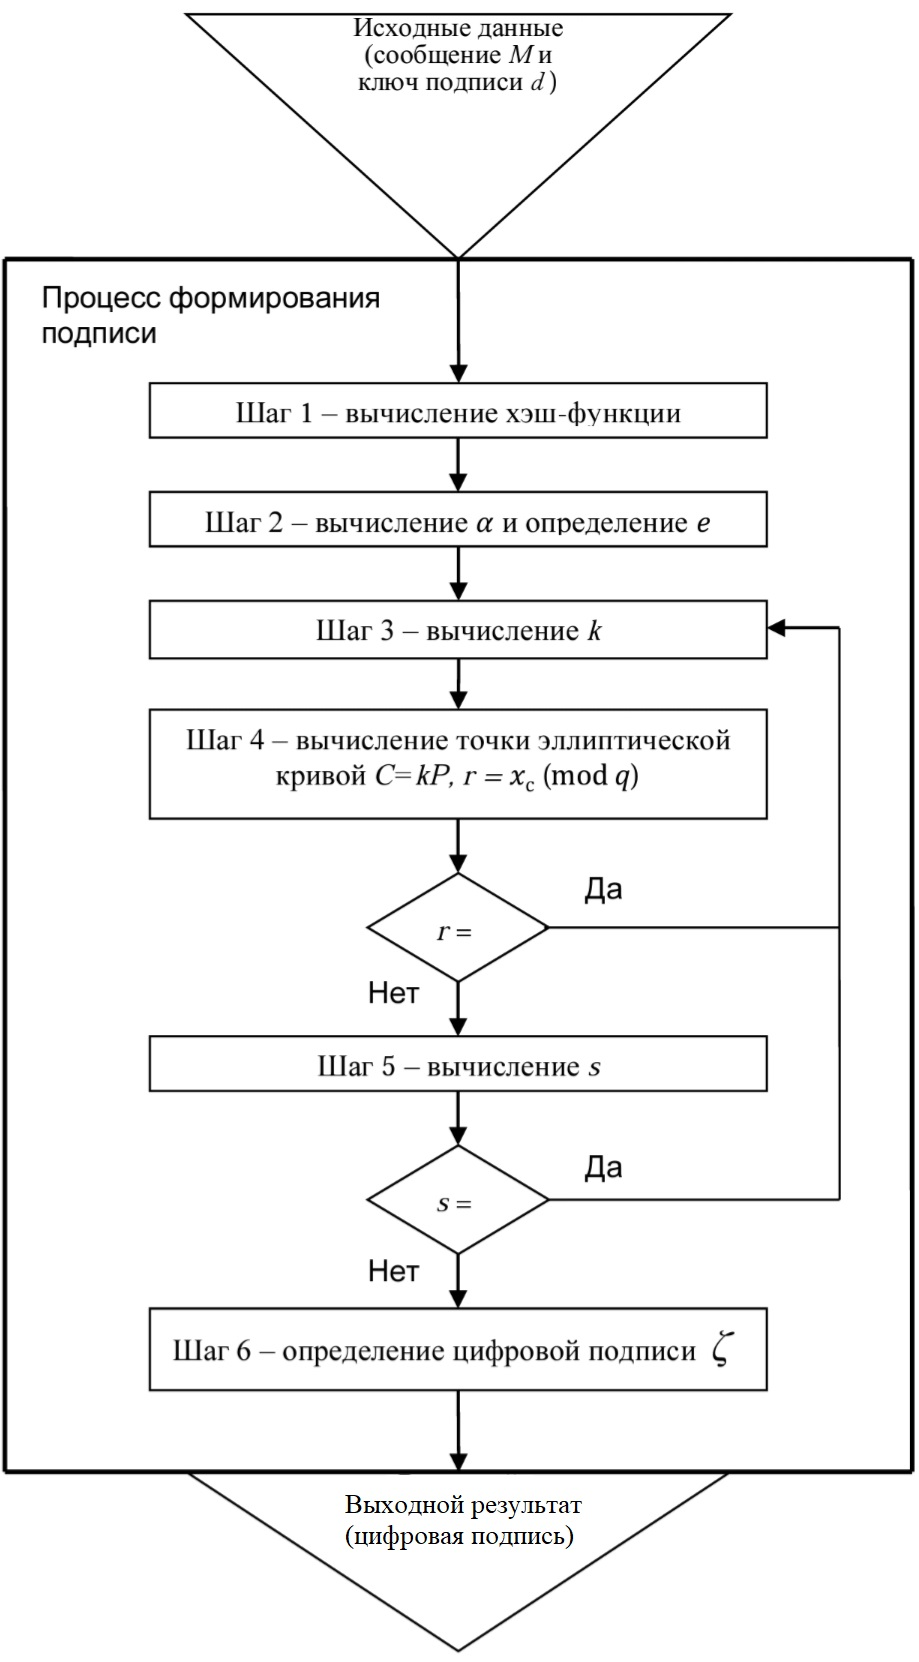
\includegraphics[width=0.62\linewidth]{inc/img/4_1}
	\caption{Схема процесса формирования ЭЦП}
	\label{fig:fig4_1}
\end{figure}

\section{Проверка подписи}
\par
Для реализации процесса проверки цифровой подписи, должны быть известны параметры схемы цифровой подписи (пункт 4.3). Исходными данными процесса являются подписанное сообщение $M$, цифровая подпись $\zeta$ и ключ проверки подписи Q, а выходным "--- свидетельство достоверности подписи.
\par
Для проверки цифровой подписи $\zeta$ под полученным сообщением $M$ необходимо выполнить следующие шаги по алгоритму II:
\par
Шаг 1 "--- по полученной подписи $\zeta$ вычислить целые числа $r$ и $s$.  Если выполнены неравенства $0<r<q$, $0<s<q$, то перейти к шагу 2. В противном случае подпись неверна.
\par
Шаг 2 "--- вычислить хэш-код полученного сообщения $M$
\begin{equation*}
\overline{h} = h(M).
\end{equation*}
\par
Шаг 3 "--- вычислить целое число $\alpha$, представлением которого является вектор $\overline{h}$ и определить
\begin{equation*}
e\equiv \alpha\;(mod\;q).
\end{equation*}
\par
Если $e=0$, то определить $e=1$.
\par
Шаг 4 "--- вычислить значение $v \equiv e^{-1}\;(mod\; q)$.
\par
Шаг 5 "--- вычислить значения
\begin{equation*}
z_1\equiv sv\;(mod\;q),\; z_2\equiv -rv\;(mod\;q).
\end{equation*}
\par
Шаг 6 "--- вычислить точку эллиптической кривой $C = z_1P+z_2Q$ и определить
\begin{equation*}
R\equiv x_c(mod\;q),
\end{equation*}
где $x_c$ "--- $x$-координата точки $C$.
\par
Шаг 7 "--- если выполнено равенство $R=r$, то подпись принимается, в противном случае - подпись неверна.
\par
Схема процесса проверки ЭЦП приведена на рисунке \ref{fig:fig4_2}.
\begin{figure}[H]
	\centering
	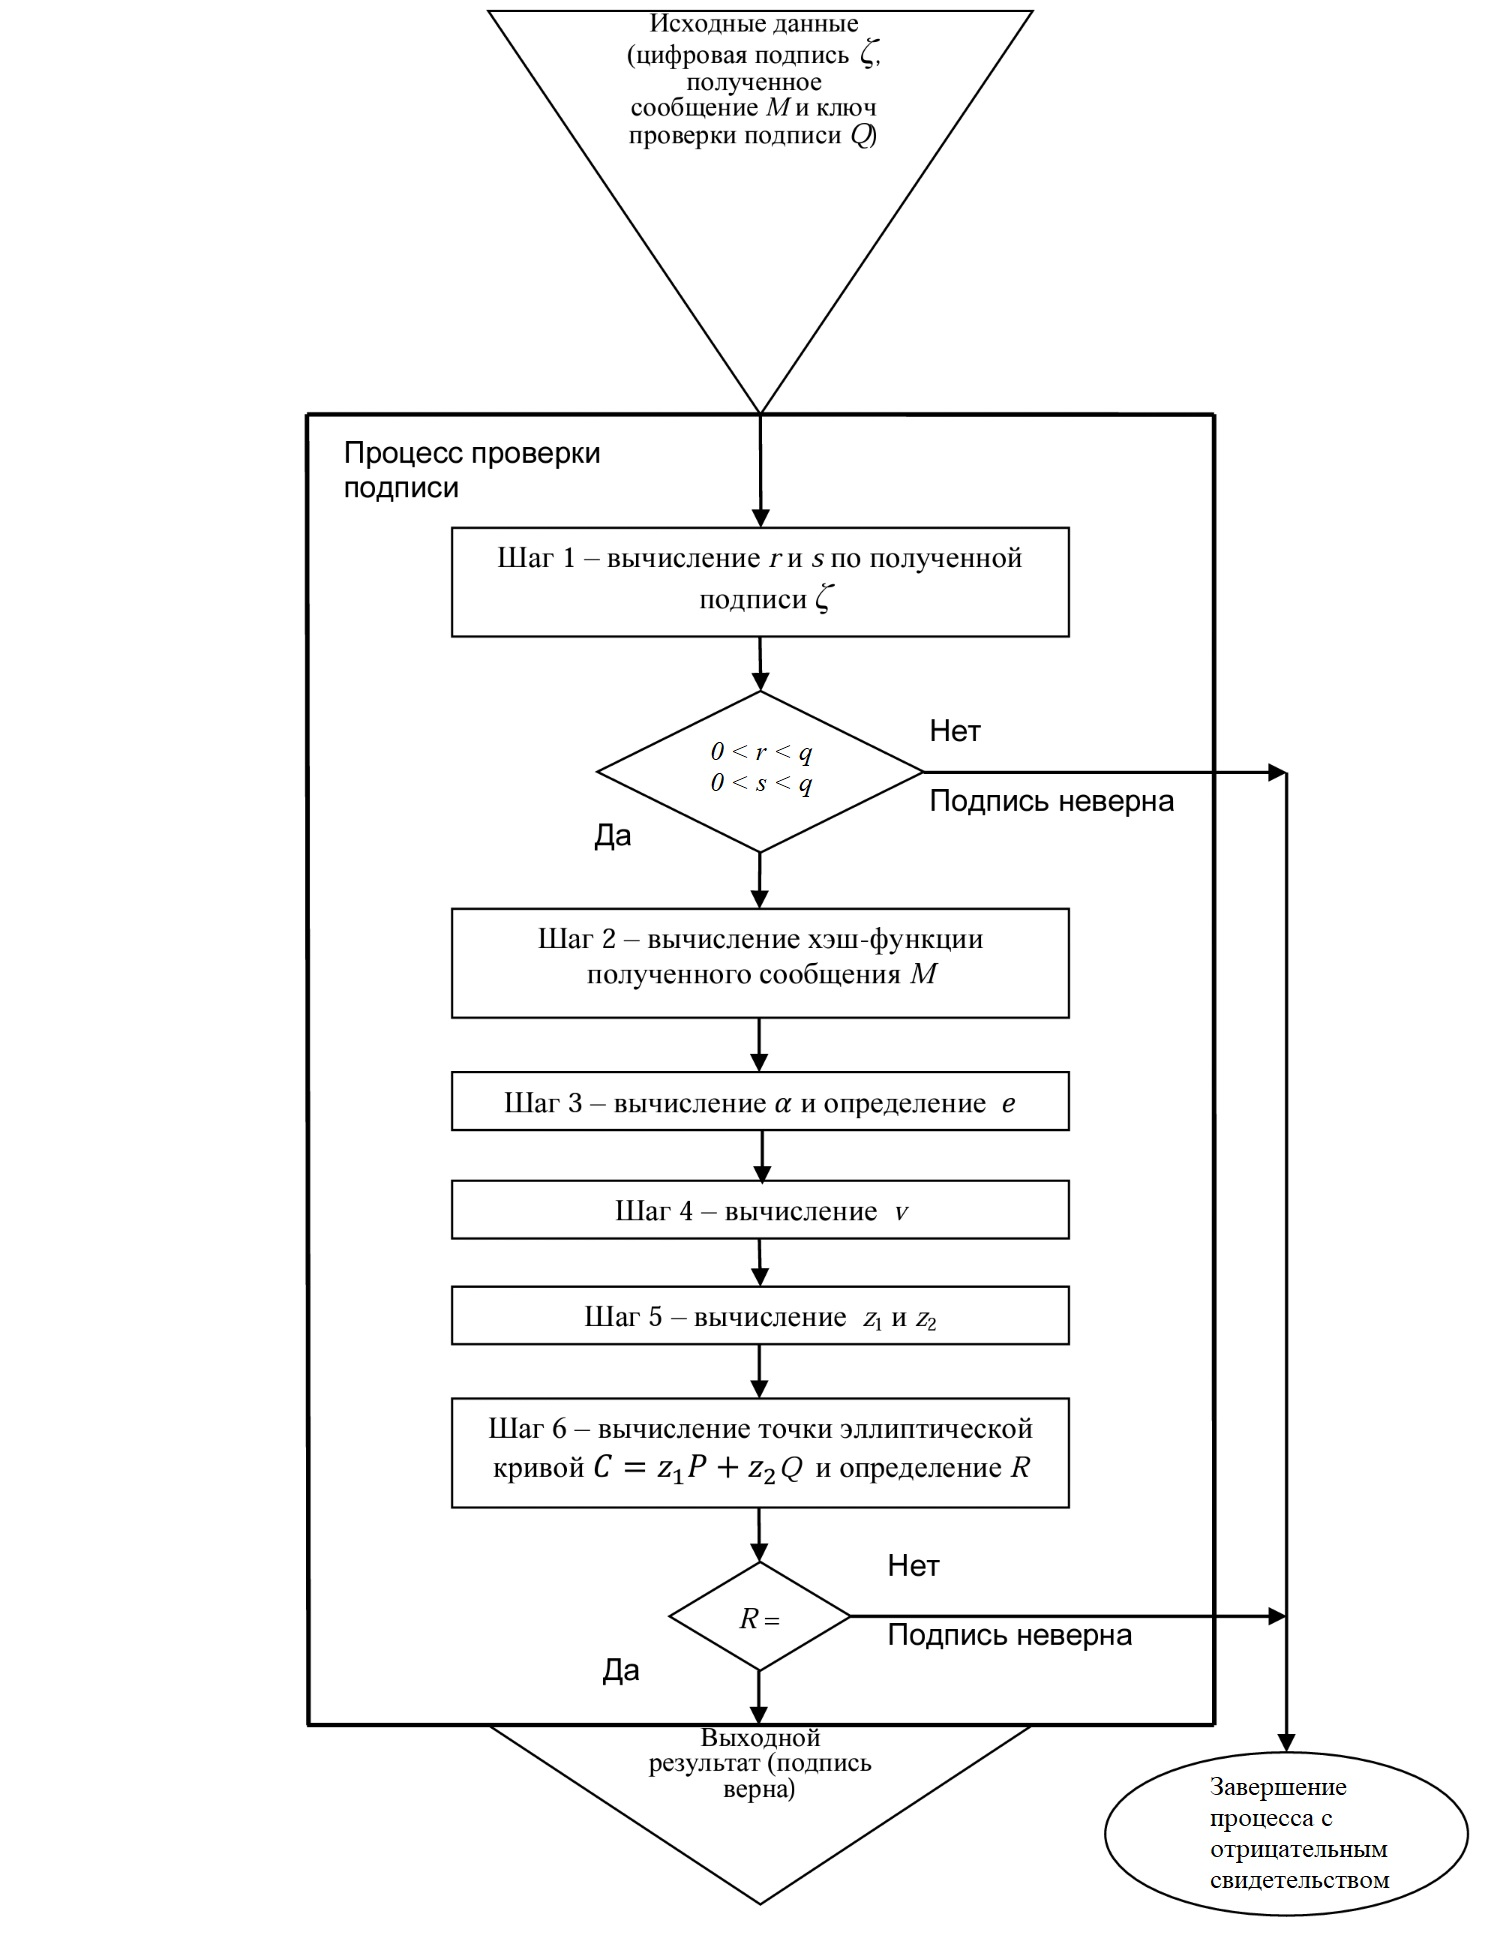
\includegraphics[width=1.0\linewidth]{inc/img/4_2}
	\caption{Схема процесса проверки ЭЦП}
	\label{fig:fig4_2}
\end{figure}